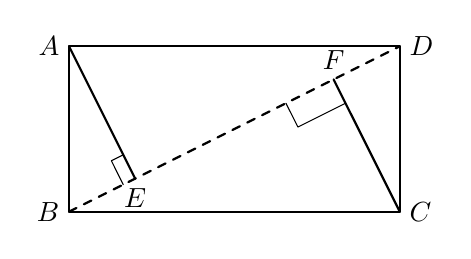
\begin{tikzpicture}[line cap=round,line join=round,scale=0.7]
\usetikzlibrary{calc}

% rectangle (wide)
\coordinate (B) at (0,0);
\coordinate (C) at (6,0);
\coordinate (D) at (6,3);
\coordinate (A) at (0,3);

\draw[thick] (A)--(B)--(C)--(D)--cycle;

% diagonal BD
\draw[dashed,thick] (B)--(D);

% feet E from A to BD, F from C to BD
\coordinate (E) at ($(B)!(A)!(D)$);
\coordinate (F) at ($(B)!(C)!(D)$);

\draw[thick] (A)--(E);
\draw[thick] (C)--(F);

% right angle marks at E and F w.r.t BD
\begin{scope}
  \coordinate (e1) at ($(E)!0.18!(B)$);
  \coordinate (e2) at ($(E)!0.18!(A)$);
  \coordinate (e3) at ($(e2)+(e1)-(E)$);
  \draw (e1) -- (e3) -- (e2);
\end{scope}
\begin{scope}
  \coordinate (f1) at ($(F)!0.18!(B)$);
  \coordinate (f2) at ($(F)!0.18!(C)$);
  \coordinate (f3) at ($(f2)+(f1)-(F)$);
  \draw (f1) -- (f3) -- (f2);
\end{scope}

% labels
\node[left] at (A) {$A$};
\node[left] at (B) {$B$};
\node[right] at (C) {$C$};
\node[right] at (D) {$D$};
\node[below] at (E) {$E$};
\node[above] at (F) {$F$};

\end{tikzpicture}